\begin{mainquestion}{nmosbias}{NMOS Bias Point Calculation}

Consider the circuit below, where $k_{n} = 3.8\ \frac{\text{mA}}{V^{2}}$ and $V_{tn} = \qty{0.5}{\volt}$.

\begin{center}
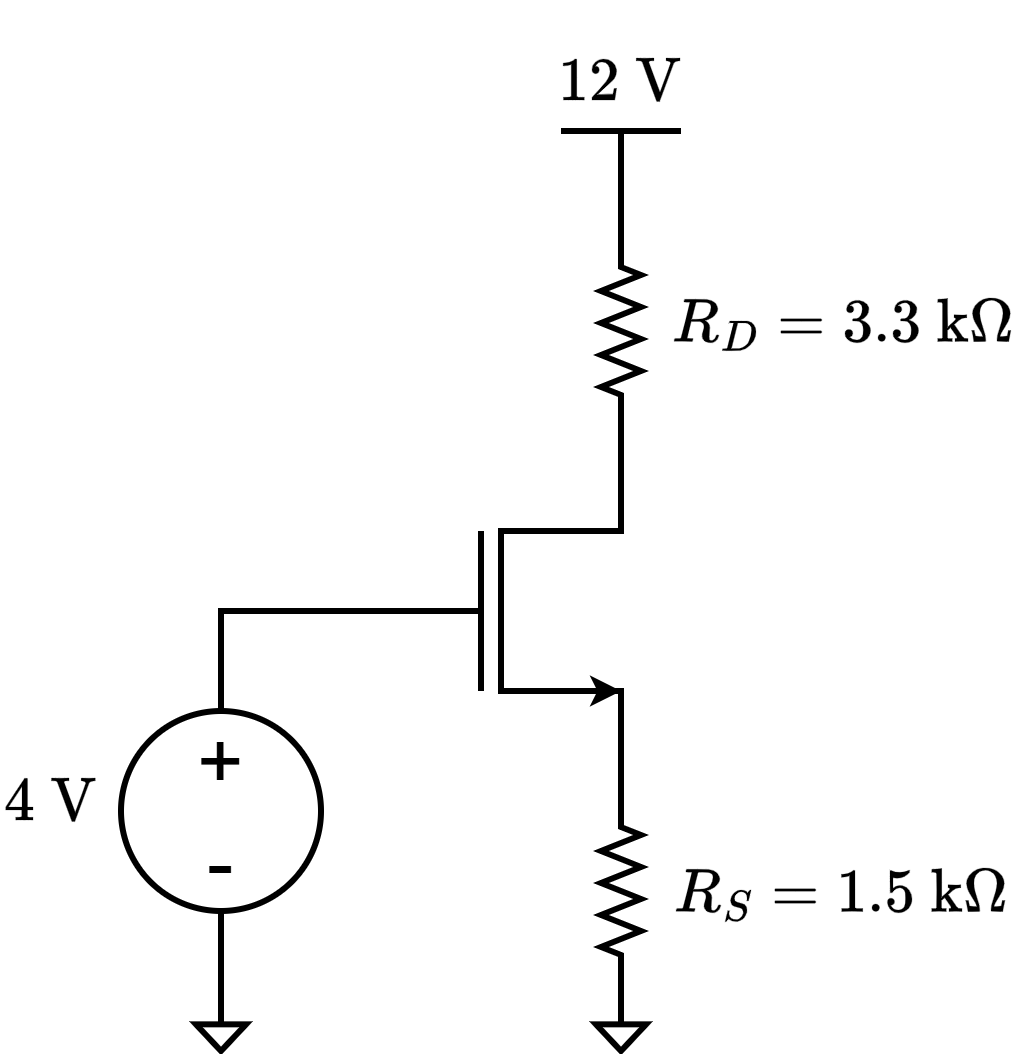
\includegraphics[height=4in]{circuit.png}
\end{center}

\begin{partquestion}{findvs}{Find the drain and source voltages for the circuit.}
\begin{answer}
We make an assumption that we are operating in the saturation region, and if we find a contradiction, we will adjust our assumption. The current $i_{D}$ (we will measure in mA) flows from drain to source in NMOS, so we expect the same current through $R_{D}$ and $R_{S}$. We then have:

\[
i_{D} = \frac{V_{DD} - V_{D}}{3.3} = \frac{V_{S} - 0}{1.5}
\]

We also know in saturation, the current is given as:

\begin{align*}
    i_D &= \frac{1}{2} k_n (v_{GS} - V_{t})^2 \\
    &= \frac{1}{2} k_n (v_G - V_S - V_{t})^2 \\
    &= \frac{1}{2} (3.8) (4 - V_S - 0.5)^2 \\
    &= (1.9)(3.5 - V_S)^2 \\
\end{align*}

Since $i_{D} = \frac{2}{3}V_{S}$, we can write:

\begin{align*}
    \frac{2}{3}V_S &= (1.9)(3.5 - V_S)^2 \\
    &= 23.275 - 13.3V_S + 1.9V_S^2 \\
    0 &= 23.275 -13.97V_S + 1.9V_S^2
\end{align*}
which has two possible solutions, $V_{S} = \qty{2.553}{\volt}$ and $V_{S} = \qty{4.797}{\volt}$. We can ignore the second solution since this would require that $v_{GS} - V_T = 4 - 4.797 - 0.5 = -1.3$. This would imply cutoff, which is not consistent with our assumption that the circuit was operating in saturation. What about the first solution? In this case $V_{OV} = 4 - 2.553 - 0.5 = 0.947$. Seems reasonable. In saturation, we have a condition that $v_{DS} > v_{GS} - V_{t}$ that we will want to validate. Since $V_{D} = V_{DD} - (\qty{3.3}{\kilo\ohm})i_D = V_{DD} - \frac{3.3}{1.5}V_S$, this results in $V_{D} = \qty{6.383}{\volt}$. Now we can compute that $v_{DS} = V_{D} - V_{S} = 6.383 - 2.553 = \qty{3.83}{\volt}$. This is a valid solution for saturation since $3.83 > 0.947$. Hence $V_{D} = \qty{6.383}{\volt}$ and $V_{S} = \qty{2.553}{\volt}$ are the bias points.
\end{answer}
\end{partquestion}

\begin{partquestion}{findcurrents}{Find the gate current and the drain current for the circuit under the same operating conditions.}
\begin{answer}
We expect no gate current in a MOSFET, so $i_{G} = 0$. For the drain current:

\[
i_{D} = \frac{V_{S}}{1.5} = \frac{\qty{2.553}{\volt}}{\qty{1.5}{\kilo\ohm}} = 1.702 \approx \qty{1.7}{\milli\ampere}.
\]
\end{answer}
\end{partquestion}

\end{mainquestion}
